\begin{figure}[H]
    \centering
    \tikzset{every picture/.style={line width=0.75pt}} %set default line width to 0.75pt
    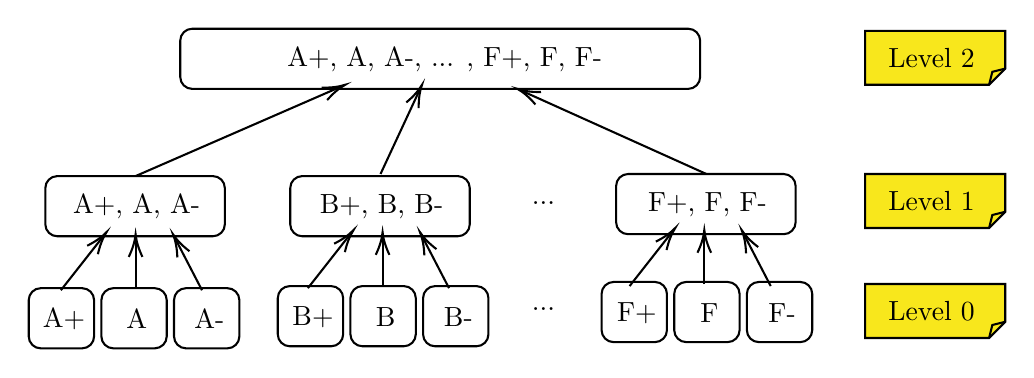
\begin{tikzpicture}[x=0.75pt,y=0.75pt,yscale=-1,xscale=1]
        %uncomment if require: \path (0,457); %set diagram left start at 0, and has height of 457

        %Rounded Rect [id:dp05055633926904224]
        \draw   (40,265.8) .. controls (40,262.6) and (42.6,260) .. (45.8,260) -- (120.7,260) .. controls (123.9,260) and (126.5,262.6) .. (126.5,265.8) -- (126.5,283.2) .. controls (126.5,286.4) and (123.9,289) .. (120.7,289) -- (45.8,289) .. controls (42.6,289) and (40,286.4) .. (40,283.2) -- cycle ;

        %Rounded Rect [id:dp15417219044870833]
        \draw   (158,265.8) .. controls (158,262.6) and (160.6,260) .. (163.8,260) -- (238.7,260) .. controls (241.9,260) and (244.5,262.6) .. (244.5,265.8) -- (244.5,283.2) .. controls (244.5,286.4) and (241.9,289) .. (238.7,289) -- (163.8,289) .. controls (160.6,289) and (158,286.4) .. (158,283.2) -- cycle ;

        %Rounded Rect [id:dp5566983339728413]
        \draw   (315,264.8) .. controls (315,261.6) and (317.6,259) .. (320.8,259) -- (395.7,259) .. controls (398.9,259) and (401.5,261.6) .. (401.5,264.8) -- (401.5,282.2) .. controls (401.5,285.4) and (398.9,288) .. (395.7,288) -- (320.8,288) .. controls (317.6,288) and (315,285.4) .. (315,282.2) -- cycle ;

        %Rounded Rect [id:dp14128108650523874]
        \draw   (32,319.8) .. controls (32,316.6) and (34.6,314) .. (37.8,314) -- (57.7,314) .. controls (60.9,314) and (63.5,316.6) .. (63.5,319.8) -- (63.5,337.2) .. controls (63.5,340.4) and (60.9,343) .. (57.7,343) -- (37.8,343) .. controls (34.6,343) and (32,340.4) .. (32,337.2) -- cycle ;

        %Rounded Rect [id:dp6850532710750563]
        \draw   (67,319.8) .. controls (67,316.6) and (69.6,314) .. (72.8,314) -- (92.7,314) .. controls (95.9,314) and (98.5,316.6) .. (98.5,319.8) -- (98.5,337.2) .. controls (98.5,340.4) and (95.9,343) .. (92.7,343) -- (72.8,343) .. controls (69.6,343) and (67,340.4) .. (67,337.2) -- cycle ;
        %Rounded Rect [id:dp49831794890726244]
        \draw   (102,319.8) .. controls (102,316.6) and (104.6,314) .. (107.8,314) -- (127.7,314) .. controls (130.9,314) and (133.5,316.6) .. (133.5,319.8) -- (133.5,337.2) .. controls (133.5,340.4) and (130.9,343) .. (127.7,343) -- (107.8,343) .. controls (104.6,343) and (102,340.4) .. (102,337.2) -- cycle ;
        %Rounded Rect [id:dp5034621708150937]
        \draw   (152,318.8) .. controls (152,315.6) and (154.6,313) .. (157.8,313) -- (177.7,313) .. controls (180.9,313) and (183.5,315.6) .. (183.5,318.8) -- (183.5,336.2) .. controls (183.5,339.4) and (180.9,342) .. (177.7,342) -- (157.8,342) .. controls (154.6,342) and (152,339.4) .. (152,336.2) -- cycle ;
        %Rounded Rect [id:dp4304422122223639]
        \draw   (187,318.8) .. controls (187,315.6) and (189.6,313) .. (192.8,313) -- (212.7,313) .. controls (215.9,313) and (218.5,315.6) .. (218.5,318.8) -- (218.5,336.2) .. controls (218.5,339.4) and (215.9,342) .. (212.7,342) -- (192.8,342) .. controls (189.6,342) and (187,339.4) .. (187,336.2) -- cycle ;
        %Rounded Rect [id:dp8079993361963536]
        \draw   (222,318.8) .. controls (222,315.6) and (224.6,313) .. (227.8,313) -- (247.7,313) .. controls (250.9,313) and (253.5,315.6) .. (253.5,318.8) -- (253.5,336.2) .. controls (253.5,339.4) and (250.9,342) .. (247.7,342) -- (227.8,342) .. controls (224.6,342) and (222,339.4) .. (222,336.2) -- cycle ;
        %Rounded Rect [id:dp3763444142614236]
        \draw   (308,316.8) .. controls (308,313.6) and (310.6,311) .. (313.8,311) -- (333.7,311) .. controls (336.9,311) and (339.5,313.6) .. (339.5,316.8) -- (339.5,334.2) .. controls (339.5,337.4) and (336.9,340) .. (333.7,340) -- (313.8,340) .. controls (310.6,340) and (308,337.4) .. (308,334.2) -- cycle ;
        %Rounded Rect [id:dp025410635634430356]
        \draw   (343,316.8) .. controls (343,313.6) and (345.6,311) .. (348.8,311) -- (368.7,311) .. controls (371.9,311) and (374.5,313.6) .. (374.5,316.8) -- (374.5,334.2) .. controls (374.5,337.4) and (371.9,340) .. (368.7,340) -- (348.8,340) .. controls (345.6,340) and (343,337.4) .. (343,334.2) -- cycle ;
        %Rounded Rect [id:dp6345478019954871]
        \draw   (378,316.8) .. controls (378,313.6) and (380.6,311) .. (383.8,311) -- (403.7,311) .. controls (406.9,311) and (409.5,313.6) .. (409.5,316.8) -- (409.5,334.2) .. controls (409.5,337.4) and (406.9,340) .. (403.7,340) -- (383.8,340) .. controls (380.6,340) and (378,337.4) .. (378,334.2) -- cycle ;
        %Rounded Rect [id:dp5704093284694525]
        \draw   (105,194.8) .. controls (105,191.6) and (107.6,189) .. (110.8,189) -- (349.7,189) .. controls (352.9,189) and (355.5,191.6) .. (355.5,194.8) -- (355.5,212.2) .. controls (355.5,215.4) and (352.9,218) .. (349.7,218) -- (110.8,218) .. controls (107.6,218) and (105,215.4) .. (105,212.2) -- cycle ;
        %Straight Lines [id:da5982931753916951]
        \draw    (47.5,315) -- (68.26,288.57) ;
        \draw [shift={(69.5,287)}, rotate = 488.16] [color={rgb, 255:red, 0; green, 0; blue, 0 }  ][line width=0.75]    (10.93,-3.29) .. controls (6.95,-1.4) and (3.31,-0.3) .. (0,0) .. controls (3.31,0.3) and (6.95,1.4) .. (10.93,3.29)   ;

        %Straight Lines [id:da7014066905322178]
        \draw    (83.5,314) -- (83.5,290) ;
        \draw [shift={(83.5,288)}, rotate = 450] [color={rgb, 255:red, 0; green, 0; blue, 0 }  ][line width=0.75]    (10.93,-3.29) .. controls (6.95,-1.4) and (3.31,-0.3) .. (0,0) .. controls (3.31,0.3) and (6.95,1.4) .. (10.93,3.29)   ;

        %Straight Lines [id:da7237438732675705]
        \draw    (115.5,315) -- (102.42,289.78) ;
        \draw [shift={(101.5,288)}, rotate = 422.59000000000003] [color={rgb, 255:red, 0; green, 0; blue, 0 }  ][line width=0.75]    (10.93,-3.29) .. controls (6.95,-1.4) and (3.31,-0.3) .. (0,0) .. controls (3.31,0.3) and (6.95,1.4) .. (10.93,3.29)   ;

        %Straight Lines [id:da9667373614001253]
        \draw    (166.5,314) -- (187.26,287.57) ;
        \draw [shift={(188.5,286)}, rotate = 488.16] [color={rgb, 255:red, 0; green, 0; blue, 0 }  ][line width=0.75]    (10.93,-3.29) .. controls (6.95,-1.4) and (3.31,-0.3) .. (0,0) .. controls (3.31,0.3) and (6.95,1.4) .. (10.93,3.29)   ;

        %Straight Lines [id:da4011582897955388]
        \draw    (202.5,313) -- (202.5,289) ;
        \draw [shift={(202.5,287)}, rotate = 450] [color={rgb, 255:red, 0; green, 0; blue, 0 }  ][line width=0.75]    (10.93,-3.29) .. controls (6.95,-1.4) and (3.31,-0.3) .. (0,0) .. controls (3.31,0.3) and (6.95,1.4) .. (10.93,3.29)   ;

        %Straight Lines [id:da5300154790184455]
        \draw    (234.5,314) -- (221.42,288.78) ;
        \draw [shift={(220.5,287)}, rotate = 422.59000000000003] [color={rgb, 255:red, 0; green, 0; blue, 0 }  ][line width=0.75]    (10.93,-3.29) .. controls (6.95,-1.4) and (3.31,-0.3) .. (0,0) .. controls (3.31,0.3) and (6.95,1.4) .. (10.93,3.29)   ;

        %Straight Lines [id:da49332566002225353]
        \draw    (321.5,313) -- (342.26,286.57) ;
        \draw [shift={(343.5,285)}, rotate = 488.16] [color={rgb, 255:red, 0; green, 0; blue, 0 }  ][line width=0.75]    (10.93,-3.29) .. controls (6.95,-1.4) and (3.31,-0.3) .. (0,0) .. controls (3.31,0.3) and (6.95,1.4) .. (10.93,3.29)   ;

        %Straight Lines [id:da6387699678510084]
        \draw    (357.5,312) -- (357.5,288) ;
        \draw [shift={(357.5,286)}, rotate = 450] [color={rgb, 255:red, 0; green, 0; blue, 0 }  ][line width=0.75]    (10.93,-3.29) .. controls (6.95,-1.4) and (3.31,-0.3) .. (0,0) .. controls (3.31,0.3) and (6.95,1.4) .. (10.93,3.29)   ;

        %Straight Lines [id:da7454255088680426]
        \draw    (389.5,313) -- (376.42,287.78) ;
        \draw [shift={(375.5,286)}, rotate = 422.59000000000003] [color={rgb, 255:red, 0; green, 0; blue, 0 }  ][line width=0.75]    (10.93,-3.29) .. controls (6.95,-1.4) and (3.31,-0.3) .. (0,0) .. controls (3.31,0.3) and (6.95,1.4) .. (10.93,3.29)   ;

        %Straight Lines [id:da41690437548834924]
        \draw    (83.5,260) -- (182.67,216.8) ;
        \draw [shift={(184.5,216)}, rotate = 516.46] [color={rgb, 255:red, 0; green, 0; blue, 0 }  ][line width=0.75]    (10.93,-3.29) .. controls (6.95,-1.4) and (3.31,-0.3) .. (0,0) .. controls (3.31,0.3) and (6.95,1.4) .. (10.93,3.29)   ;

        %Straight Lines [id:da9088806507789935]
        \draw    (201.5,259) -- (220.66,217.81) ;
        \draw [shift={(221.5,216)}, rotate = 474.94] [color={rgb, 255:red, 0; green, 0; blue, 0 }  ][line width=0.75]    (10.93,-3.29) .. controls (6.95,-1.4) and (3.31,-0.3) .. (0,0) .. controls (3.31,0.3) and (6.95,1.4) .. (10.93,3.29)   ;

        %Straight Lines [id:da6354688861477524]
        \draw    (358.5,259) -- (269.32,218.82) ;
        \draw [shift={(267.5,218)}, rotate = 384.25] [color={rgb, 255:red, 0; green, 0; blue, 0 }  ][line width=0.75]    (10.93,-3.29) .. controls (6.95,-1.4) and (3.31,-0.3) .. (0,0) .. controls (3.31,0.3) and (6.95,1.4) .. (10.93,3.29)   ;

        %Shape: Folded Corner [id:dp6484816765083135]
        \draw  [fill={rgb, 255:red, 248; green, 231; blue, 28 }  ,fill opacity=1 ] (494.7,338) -- (435,338) -- (435,312) -- (502.5,312) -- (502.5,330.2) -- cycle -- (494.7,338) ; \draw   (502.5,330.2) -- (496.26,331.76) -- (494.7,338) ;
        %Shape: Folded Corner [id:dp9570029764461927]
        \draw  [fill={rgb, 255:red, 248; green, 231; blue, 28 }  ,fill opacity=1 ] (494.7,285) -- (435,285) -- (435,259) -- (502.5,259) -- (502.5,277.2) -- cycle -- (494.7,285) ; \draw   (502.5,277.2) -- (496.26,278.76) -- (494.7,285) ;
        %Shape: Folded Corner [id:dp38314853861140774]
        \draw  [fill={rgb, 255:red, 248; green, 231; blue, 28 }  ,fill opacity=1 ] (494.7,216) -- (435,216) -- (435,190) -- (502.5,190) -- (502.5,208.2) -- cycle -- (494.7,216) ; \draw   (502.5,208.2) -- (496.26,209.76) -- (494.7,216) ;

        % Text Node
        \draw (84,275) node  [align=left] {A+, A, A-};
        % Text Node
        \draw (202,275) node  [align=left] {B+, B, B-};
        % Text Node
        \draw (359,274) node  [align=left] {F+, F, F-};
        % Text Node
        \draw (280,273) node  [align=left] {...};
        % Text Node
        \draw (49,329) node  [align=left] {A+};
        % Text Node
        \draw (84,329) node  [align=left] {A};
        % Text Node
        \draw (119,329) node  [align=left] {A-};
        % Text Node
        \draw (204,328) node  [align=left] {B};
        % Text Node
        \draw (239,328) node  [align=left] {B-};
        % Text Node
        \draw (169,328) node  [align=left] {B+};
        % Text Node
        \draw (360,326) node  [align=left] {F};
        % Text Node
        \draw (395,326) node  [align=left] {F-};
        % Text Node
        \draw (325,326) node  [align=left] {F+};
        % Text Node
        \draw (280,324) node  [align=left] {...};
        % Text Node
        \draw (232.42,204) node  [align=left] {A+, A, A-, ... , F+, F, F-};
        % Text Node
        \draw (467,325) node  [align=left] {Level 0};
        % Text Node
        \draw (467,272) node  [align=left] {Level 1};
        % Text Node
        \draw (467,203) node  [align=left] {Level 2};


    \end{tikzpicture}
    \caption{Generalization hierarchy for school grades}\label{fig:grades-hierarchy}
\end{figure}